\documentclass[a4paper, top=10mm]{article}
%for writing from the top
\usepackage{fullpage}
%for math
\usepackage{amsmath}
\usepackage{mathrsfs}
\usepackage{amsthm}
%for images
\usepackage{graphicx}
%for color
\usepackage{xcolor}
%for title
\title{\textbf{\huge{Crofto(w)n}}}
\author{Enigma n\textsuperscript{o}2}
\date{2\textsuperscript{nd} December 2022}

\newtheorem*{hint}{Hint}

\addtolength{\voffset}{-2cm}
\addtolength{\textheight}{5cm}


\begin{document}
	\maketitle
	
	A mathematician, is visiting a new city: Crofto(w)n.
	
	He is worried: he would like to visit all the important points of this city:
	the shop (S'), the museum (M), the observation point (O), the science museum (S), the library (L), a historical monument (H), a park (P), and he would also like to take a break in a coffee shop (C).
	The order doesn't matter. As there is an art exposition in the streets, he also wants to visit all the streets of the town. To avoid getting bored, the streets have to be use exactly once.
	
	\begin{center}
		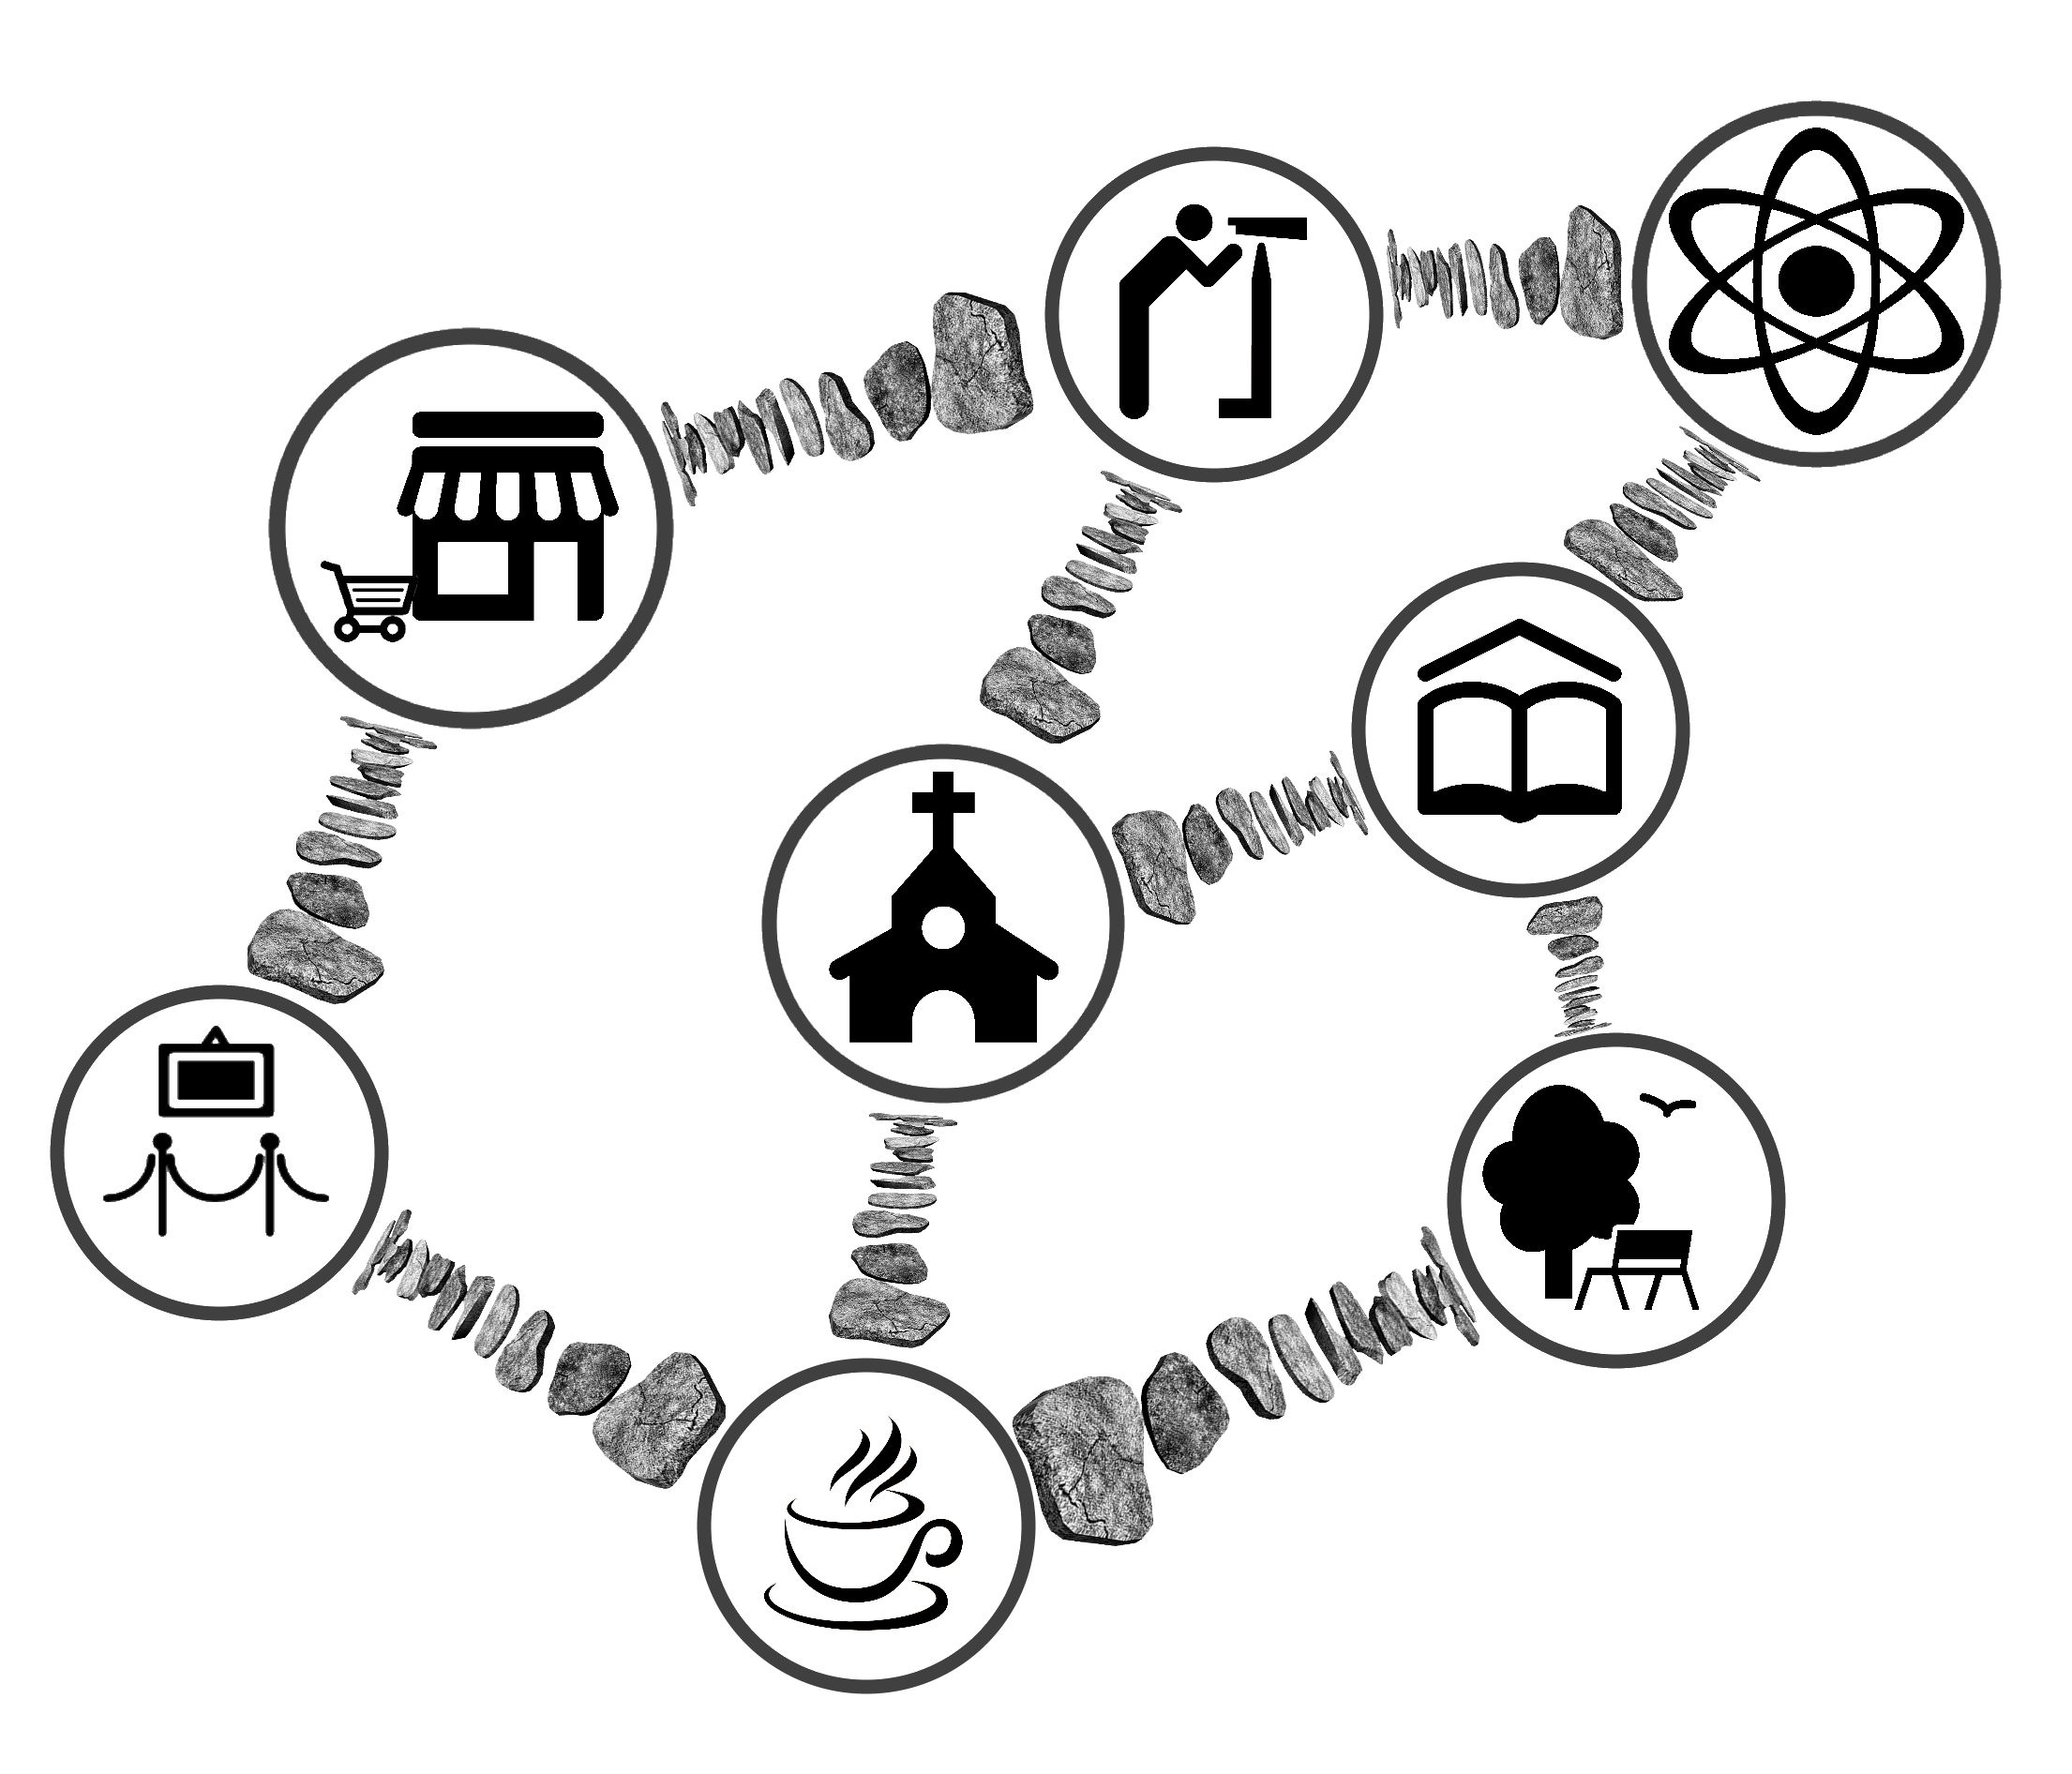
\includegraphics[height=270pt]{02city.png}\\
		Map of the town
		
		(please don't blame my graphics skills)
	\end{center}
	
	Find how many distinct paths there are for a mathematician tourist: visiting all the important points and visit all the streets of the city exactly once. 
	The mathematician arrives and leaves the city by tube, which has stations everywhere (i.e.: paths may start from anywhere you want).
	The streets may all be used both ways (no one way street).
	
	\begin{center}
		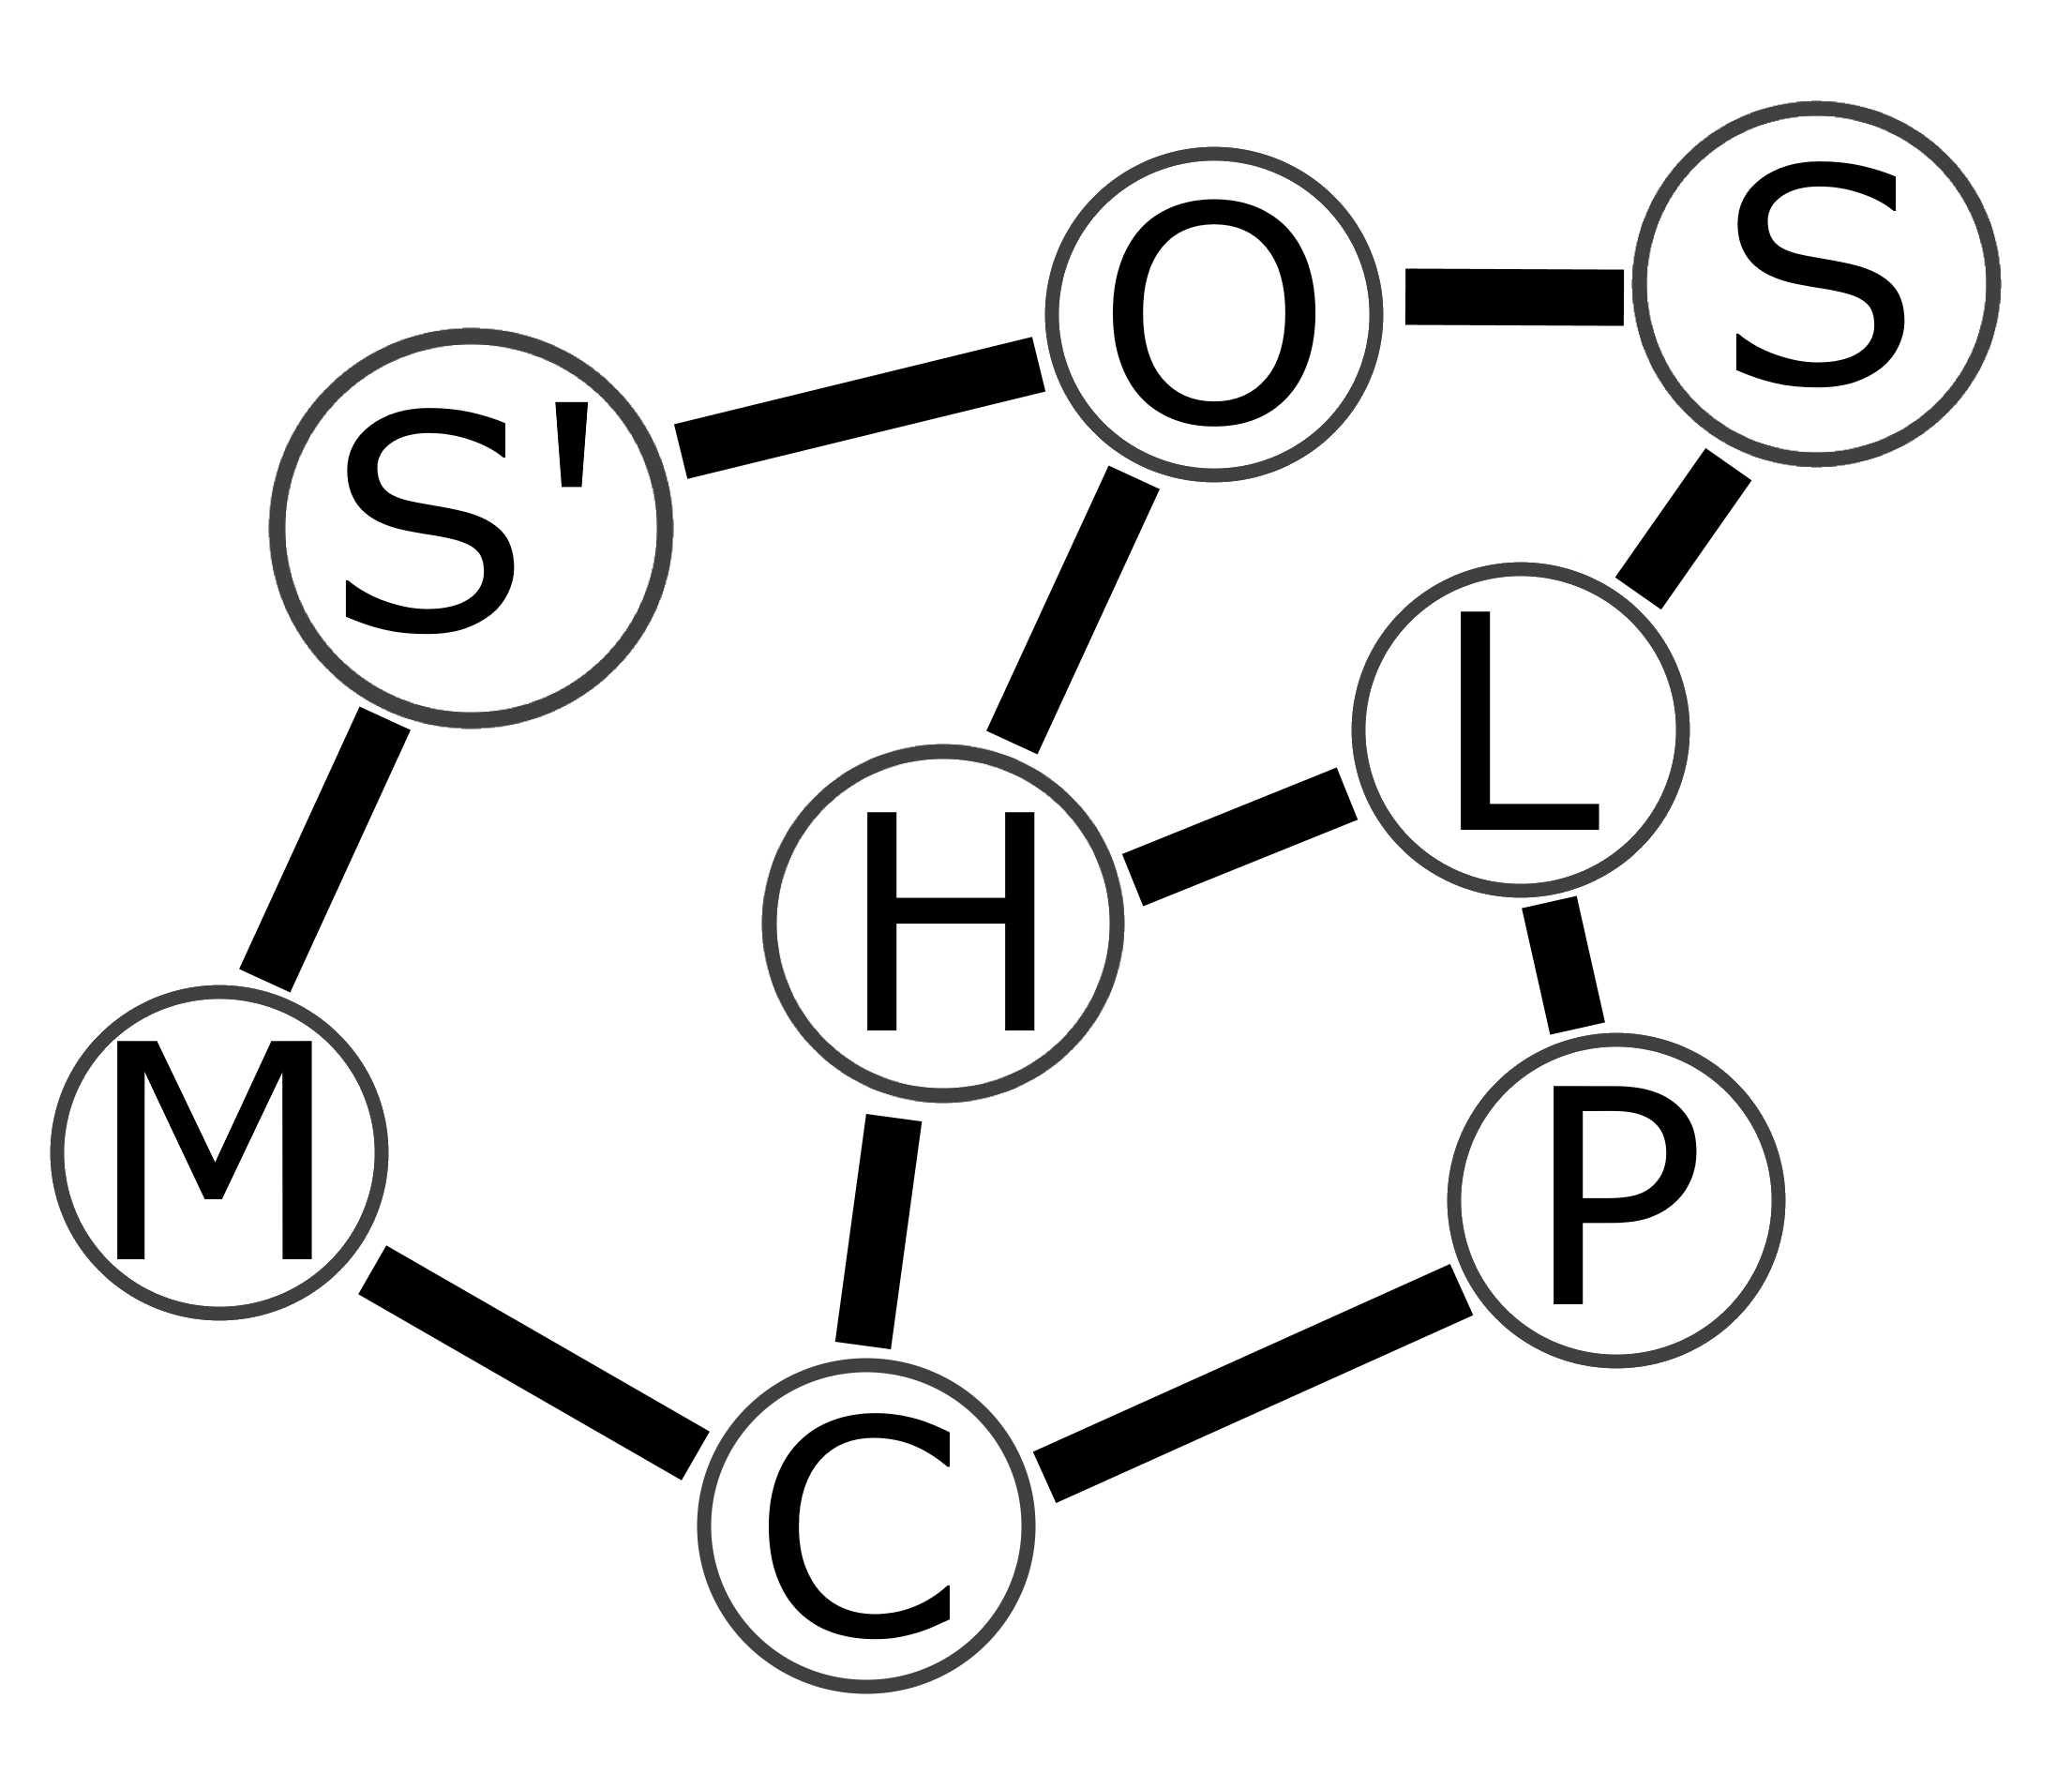
\includegraphics[height=200pt]{02graph.png}\\
		For simplicity, use the notations with letters.
	\end{center}
	
\end{document}